\setcounter{equation}{0}
Нормальной автономной системой дифференциальных уравнений порядка $n$ называется система
\begin{equation}\label{autonom-sys}
    \dot{x}(t) = f(x)
\end{equation}
где $f(x)$— заданная действительная вектор-функция c $n$ компонентами определенная в некоторой области (называется фазовым пространством автономной системы) $\Omega$ евклидового пространства $\mathbb{R}_x^n$ с
фиксированной прямоугольной декартовой системой координат $x_1, \ldots, x_n$.

В системе~(\ref{autonom-sys}) $t$~--- независимая переменная, которую принято называть временем и считать лежащей в $\mathbb{R}_t^1$, а $x(t)$~--- неизвестная действительная вектор-функция c $n$ компонентами.

В дальнейшем будем предполагать, что $f(x)$ удовлетворяет в области $\Omega$ условию Липшица. Это гарантирует существование и единственность непродолжимого решения системы~(\ref{autonom-sys}) при начальном условии
\begin{equation}\label{autonom-sys-condition}
    x(t_0) = x_0, x_0 \in \Omega,
\end{equation}
на некотором промежутке $I = I(t_0, x_0)$ оси $t$, содержащей точку $t_0$.

Произвольная нормальная система дифференциальных уравнений
\begin{equation}\label{autonom-sys-custom}
    \dot{x}(t) = f(x, t)
\end{equation}
всегда сводится к автономной системе путем увеличения числа неизвестных функций на единицу. Если положить \(t = x_{n + 1}\), то получаем автономную систему с \((n - 1)\) неизвестными функциями:
\[
 \begin{cases}
 \dot{x}(t) = f(x, x_{n + 1})\\
 \dot{x}_{n+1} = 1
 \end{cases}.
\]

Таким образом, автономная система~(\ref{autonom-sys}) отличается от любой системы~(\ref{autonom-sys-custom}) тем, что правая часть~(\ref{autonom-sys}) не содержит переменной $t$.

\begin{definition}
Если \(x = \varphi(t)\)~--- решение системы~(\ref{autonom-sys}) на промежутке \(I \subseteq \mathbb{R}_t^1\), то оно определяет параметрически заданную кривую в области $\Omega$, т.е. множество точек \(\{\varphi(t)\} \in \Omega\) при всех \(t \in I\). Эта кривая в $\Omega$ называется фазовой траекторией автономной системы~(\ref{autonom-sys}).
\end{definition}

Интегральные кривые~(\ref{autonom-sys}) представляют собой графики решений \(x = \varphi(t)\) системы~(\ref{autonom-sys}) в бесконечном цилиндре
\[G = \{(x, t) \in \mathbb{R}_{(x, t)}^{n + 1} : x \in \Omega, t \in \mathbb{R}_t^1\}\]
\((n + 1)\)\,-мерного пространства $\mathbb{R}_{(x, t)}^{n + 1}$. 

Следовательно, фазовая траектория~(\ref{autonom-sys}) является проекцией интегральной кривой~(\ref{autonom-sys}) параллельно оси $t$ (см. рис.\,\ref{fkng-cylinder}). На траектории стрелкой указывают ее ориентацию, т.е. направление движения по ней в сторону возрастания $t$.

\begin{figure}[ht]\label{fkng-cylinder}
    \centering
    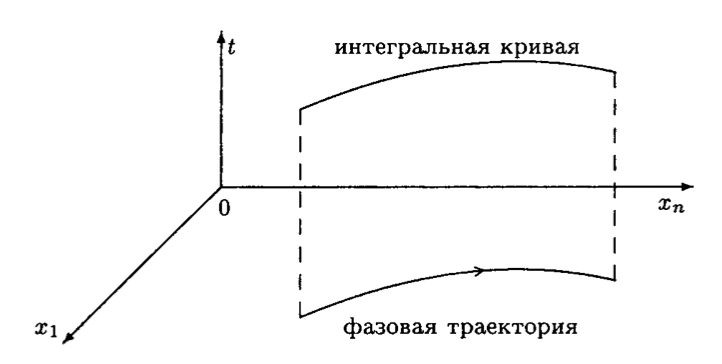
\includegraphics[scale=0.8]{sections/Sasha/images/fkng-cylinder.png}
    \caption{Цилиндр о котором речь}
\end{figure}

Из теоремы существования и единственности решения задачи Коши~(\ref{autonom-sys}),~(\ref{autonom-sys-condition}) получаем, что через каждую точку \(x_0 \in \Omega\) проходит единственная траектория~(\ref{autonom-sys}), определенная в некоторой окрестности $t_0$. При некоторых
достаточных условиях эта траектория определена при всех \(t \in \mathbb{R}_t^1\).

\paragraph{Свойства фазовых траекторий}

\begin{theorem}[очев]
Если \(x(t) = \varphi(t)\)~--- решение~(\ref{autonom-sys}) при \(t \in (\alpha ; \beta)\) и $C$~--- некоторое действительное число, то \(x(t) = \varphi(t + c)\)~--- решение при \(t \in (\alpha - c; \beta - c)\).
\end{theorem}
\begin{center}
    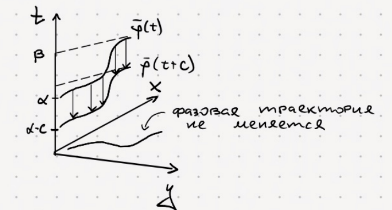
\includegraphics[width=0.5\linewidth]{images/proof.png}
\end{center}

\begin{theorem}
Если две фазовых траектории \(x(t) = \varphi(t), t \in I_1\) и \(x(t) = \psi(t), t \in I_2\)~--- решения~(\ref{autonom-sys}) и \[x_0 = \varphi(t_1) = \psi(t_2)\], то \(\psi(t) \equiv \varphi(t + t_1 - t_2)\) для всех $t$ для которых определены обе части тождества
\end{theorem}
\begin{proof}
Рассмотрим \(y = \varphi_1(t) = \varphi(t + t_1 - t_2), t + t_1 - t_2 \in I_1\), тогда
\( \varphi_1(t_2) = \varphi(t_1) = \psi(t_2)\). Из этого следует, что \(\varphi_1(t_2) =\psi(t_2) = x_0\). Но тогда по теореме существования и единственности, для всех $t$ для которых определены обе части тождества, получаем необходимое тождество.
\end{proof}

\begin{definition}
Решение системы~(\ref{autonom-sys}) \(x(t) = \varphi(t) \equiv x_0 \in \Omega, \forall t \in \mathbb{R}_t^1\) называется положением равновесия или точкой покоя системы~(\ref{autonom-sys})
\end{definition}

\begin{theorem}
Точка \(x_0 \in \Omega \) является положением равновесия системы~(\ref{autonom-sys}) тогда и только тогда когда \(f(x_0) = 0\).
\end{theorem}
\begin{proof}
\fbox{$\Longrightarrow$} Пусть \(x = x_0\)~--- п.р.~(\ref{autonom-sys}). Тогда \(\dot{x} = f(x_0) = 0\).\\
\fbox{$\Longleftarrow$} Пусть \(f(x_0) = 0\). Тогда \(\dot{x} = 0\) и \(x = x_0\).
\end{proof}

\begin{definition}
Если решение системы~(\ref{autonom-sys}) \(x = \varphi(t), \forall t \in \mathbb{R} _t^1\) и является периодической вектор-функцией с периодом $T$, то соответствующая ему фазовая траектория называется циклом системы.
\end{definition}

\begin{theorem}[б/д]
Все фазовые траектории системы~(\ref{autonom-sys}) принадлежат одному из трех классов:
\begin{enumerate}
    \item положение равновесия;
    \item замкнутая траектория (цикл);
    \item траектория без самопересечений.
\end{enumerate}
\end{theorem}
\begin{figure}[h]
    \begin{minipage}[h]{0.5\linewidth}
    Замкнутая траектория:
\begin{center}
    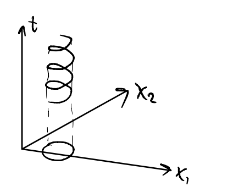
\includegraphics[width=0.5\linewidth]{images/cycle.png}
\end{center}
    \end{minipage}
    \hspace{-4ex}
    \begin{minipage}[h]{0.5\linewidth}
Иллюстрация к теореме 5.3:
\begin{center}
    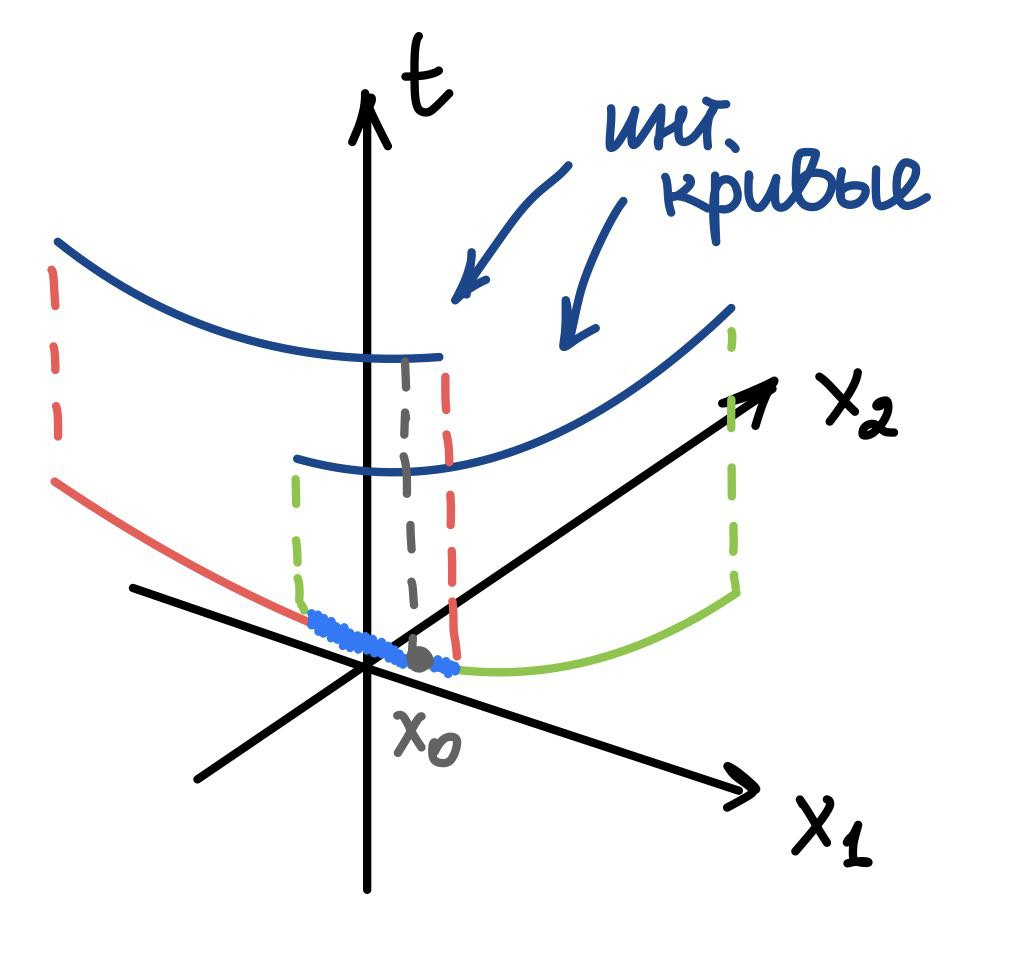
\includegraphics[width=0.5\linewidth]{images/th2.jpg}
\end{center}
    \end{minipage}
\end{figure}



